% ncse_new/\problems/ch_piecewisepolynomials/ex_CurveInterp.tex
% exercise requires:    heart.m  intpolyval.m
% solutions require:    curveintp.m  heart_Sol.m  ex_CurveIntp.eps  heart_transform.m


\begin{problem}[Curve Interpolation \coreproblem] \label{prb:CurveInterp}

The focus of \lref{cha:PolynomialInterpolation} was on the interpolation of
data points by means of functions belonging to a certain linear space. % of functions.
A different task is to find a curve containing each point of a set
$\{\mathbf{p}_0,...,\mathbf{p}_n\}\subset \mathbb{R}^2$.

This task can be translated in a standard interpolation problem after recalling
that a curve in $\bbR^{2}$ can be described by a mapping (\emph{parametrization})
$\gammabf:[0,1]\mapsto\bbR^{2}$, $\gammabf(t) = \binom{s_{1}(t)}{s_{2}(t)}$. Hence,
given the nodes $0 = t_0 < t_{1} < ... < t_{n-1} < t_n = 1$, we aim at finding interpolating
functions $s_1, s_2: [0,1] \rightarrow \mathbb{R}$, such that $s_i(t_j)
= (\mathbf{p}_j)_i$, $i=1,2$, $j=0,...,n$. This means that we separately
interpolate the $x$ and $y$ coordinates of $\mathbf{p}_j$.

A crucial new aspect is that the nodes are not fixed, i.e., there are infinitely many parameterizations for a given curve: for any strictly
monotonous and surjective $h:[0,1]\rightarrow[0,1]$ %(with $h(0)=0$ and $h(1)=1$)
the mappings $\gammabf$ and $\wt{\gammabf} :=
\gammabf\circ h$ describe exactly the same curve. On the other hand, the selection of
nodes will affect the interpolants $s_{1}$ and $s_{2}$ and leads to different
interpolating curves.

%  This problem should give you an idea of how different choices of nodes and interpolation methods lead to different interpolating curves.

Concerning the choice of the nodes, we will consider two options:
\begin{align}
  \label{eq:pte}
  \text{\ding{202}}\qquad & \text{equidistant parametrization: $t_k = k \Delta t$,
    $\Delta t = \frac{1}{n}$}\\
  \label{eq:ptl}
  \text{\ding{203}}\qquad & \text{segment length parametrization:
$\displaystyle{t_k = \frac{\sum_{l=1}^k|\mathbf{p}_l - \mathbf{p}_{l-1}|}{\sum_{l=1}^n|\mathbf{p}_l - \mathbf{p}_{l-1}|}}$}\;.
\end{align}


Point data will be generated by the \Matlab{} function \;\texttt{heart}\;  that is available on the course webpage.
%  These points should be used in all of the following sub-problems.

% ============= SUBPROBLEM 1

\begin{subproblem}[3] \label{subprb:CurveInterp_1}
Write a \Matlab{} function
%
\begin{center}
\texttt{function \quad pol = polycurveintp (xy,t,tt)}
\end{center}
%
which uses global polynomial interpolation (using the \texttt{intpolyval}
function, see \ncseref[Code]{barycentricformula}) through the $n+1$ points
$\Vp_{i}\in\bbR^{2}$, $i=0,\ldots,n$, whose coordinates are stored in the $2
\times (n+1)$ matrix \texttt{xy} and returns sampled values of the obtained curve
in a $2 \times N$ matrix \texttt{pol}.  Here, \texttt{t} passes the node vector
$(t_{0},t_{1},\ldots,t_{n})\in\bbR^{n+1}$ in the parameter domain and $N$ is the
number of equidistant sampling points.

\hint{} Code for \texttt{intpolyval} is available as \texttt{intpolyval.m}.

\begin{solution}
See \autoref{mc:curveintp}.
\lstinputlisting[caption={Matlab Code for \texttt{curveintp}},label={mc:curveintp}]
{\problems/ch_piecewisepolynomials/MATLAB/curveintp.m}
\end{solution}
\end{subproblem}

% ============= SUBPROBLEM 2

\begin{subproblem}[1] \label{subprb:CurveInterp_2}
Plot the curves obtained by global polynomial interpolation \texttt{polycurveintp}
of the \texttt{heart} data set. The nodes for polynomial interpolation should be
generated according to the two options \eqref{eq:pte} and \eqref{eq:ptl}

\begin{solution}
See \autoref{mc:heart_Sol} and \autoref{fig:ex_CurveIntp}.
\end{solution}
\end{subproblem}

% ============= SUBPROBLEM 3

\begin{subproblem}[3] \label{subprb:CurveInterp_3}
Extend your \Matlab{} function \texttt{pol = curveintp} to
%
\begin{center}
\texttt{function \quad pch = pchcurveintp (xy,t,tt)},
\end{center}
%
which has the same purpose, arguments and return values as \texttt{polycurveintp}, but now
uses monotonicity preserving cubic Hermite interpolation  (available through the
\Matlab{} built-in function \texttt{pchip}, see also \lref{sec:hipshp}) instead of global 
polynomial interpolation. 

Plot the obtained curves for the \texttt{heart} data set in the figure created in
sub-problem \ref{subprb:CurveInterp_2}. Use both parameterizations \eqref{eq:pte}
and \eqref{eq:ptl}.

\begin{solution}
See \autoref{mc:curveintp} and \autoref{fig:ex_CurveIntp}.
\end{solution}
\end{subproblem}

% ============= SUBPROBLEM 4

\begin{subproblem}[3] \label{subprb:CurveInterp_4}
Finally, write yet another \Matlab{} function 
%
\begin{center}
\texttt{function \quad spl = splinecurveintp (xy,t,tt)},
\end{center}
%
which has the same purpose, arguments and return values as \texttt{polycurveintp}, but
now uses \textit{complete} cubic spline interpolation.

The required derivatives $s_{1}'(0)$, $s_{2}'(0)$, $s_{1}'(1)$, and $s_{2}'(1)$
should be computed from the directions of the line segments connecting $\Vp_{0}$
and $\Vp_{1}$, and $\Vp_{n-1}$ and $\Vp_{n}$, respectively.  You can use the
\Matlab{} built-in function \texttt{spline}.  Plot the obtained curves
(\texttt{heart} data) in the same figure as before using both parameterizations
\eqref{eq:pte} and \eqref{eq:ptl}.

\hint{} read the \Matlab{} help page about the \texttt{spline} command and learn how to impose the derivatives at the endpoints.

\begin{solution}
The code for the interpolation of the heart:
\lstinputlisting[caption={Matlab Code for \texttt{heart\_Sol}},label={mc:heart_Sol}]
{\problems/ch_piecewisepolynomials/MATLAB/heart_Sol.m}

\begin{figure}[htb]\begin{center}
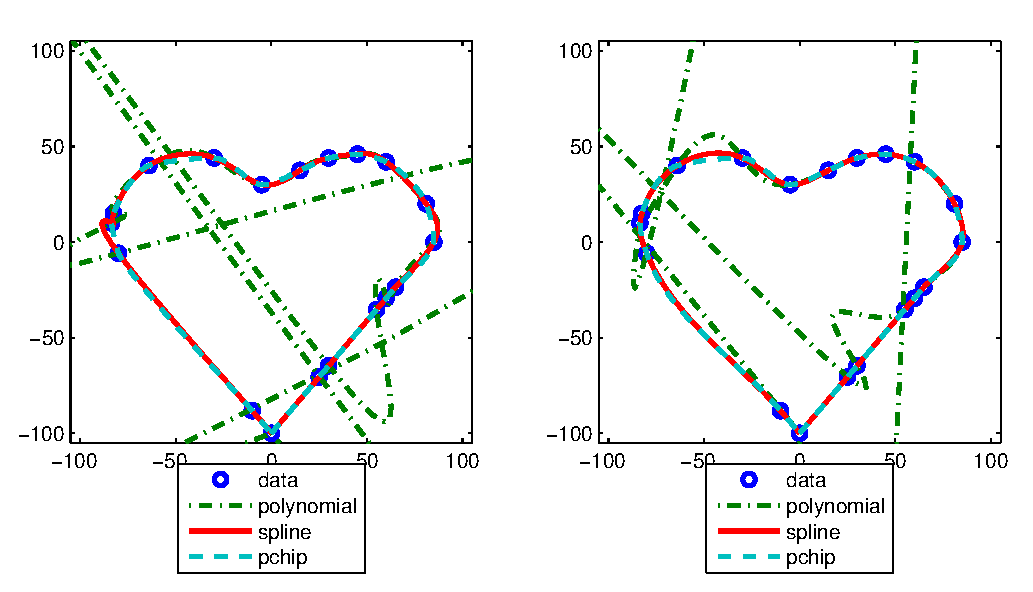
\includegraphics[width = 0.9\textwidth]{\problems/ch_piecewisepolynomials/PICTURES/ex_CurveIntp.eps}
\caption{Plots for different parametrizations and interpolation schemes}
\label{fig:ex_CurveIntp}
\end{center}\end{figure}

\textbf{Remarks:}
\begin{itemize}
 \item Note that \texttt{pchip} is a non-linear interpolation, so there is no linear mapping (matrix) from the nodes to the polynomial coefficients.
 \item Global polynomial interpolation fails. The degree of the polynomial is too high ($n$), and the typical oscillations can be observed.
 \item In this case, when two nodes are too close, spline interpolation with equidistant pa\-ra\-me\-tri\-za\-tion introduces small spurious oscillations.
\end{itemize}
\end{solution}
\end{subproblem}
\iffalse
% ============= SUBPROBLEM 5

\subproblem \label{subprb:CurveInterp_5} \difficulty{2} \pts{2}
The three interpolation schemes introduced in
subproblems~\ref{subprb:CurveInterp_1}, \ref{subprb:CurveInterp_3}, and 
\ref{subprb:CurveInterp_4} combined with either of the choices \eqref{eq:pte} and
\eqref{eq:ptl} of interpolation nodes in the parameter domain define a 
\emph{curve interpolation operator}
\begin{gather*}
  I_{\mathrm{curve}}:(\bbR^{2})^{n+1} \to \{\gamma:[0,1] \to \bbR^{2}\}\;.
\end{gather*}
Which of the six curve interpolation operators (three different interpolation
methods $\times$ two options for choosing the nodes) is linear.

\begin{solution}
Independently of the parametrization type, global polynomial and spline interpolations are linear, whereas cubic Hermite is non-linear.
}

\subproblem \label{subprb:CurveInterp_6} \difficulty{3} \pts{3}
It is interesting to study, how a transformation of the points affects the
interpolating curve:

Every linear mapping $T_A:x \mapsto \VA x$ with regular matrix $\VA \in \IR^{2,2}$
maps the plane to itself. 
%
Check experimentally whether
%
\begin{equation*}
I_{\text{curve}} ( \{ T_A \Vp_l \}_l ) = T_A I_{\text{curve}} ( \{ \Vp_l \}_l )
\end{equation*}
%
for two different matrices $A \in \{\VA_1, \VA_2\}$, given by
%
\begin{equation*}
\VA_1 =
\begin{pmatrix}
\cos(\theta) & \sin(\theta) \\
-\sin(\theta) & \cos(\theta)
\end{pmatrix}
\quad \text{with} \quad \theta = \frac{\pi}{3},
\quad \text{and} \quad
\VA_2 =
\begin{pmatrix}
1 & \lambda \\
0 & 1
\end{pmatrix}
\quad \text{with} \quad \lambda = 3, 
\end{equation*}
%
where $I_{\text{curve}} \in \{ 6 \text{ different interpolation schemes from the
  previous sub-problems} \}$. $\VA_1$ is a rotation matrix and $\VA_2$ is a shear
deformation matrix. Which matrix is orthogonal?

\begin{solution}
The code for checking whether interpolations are invariant under given linear transformations of the heart:
%
\lstinputlisting[caption={Matlab Code for \texttt{heart\_transform}},label={mc:heart_transform}]
{\problems/ch_piecewisepolynomials/MATLAB/heart_transform.m}
%
The output of \texttt{heart\_transform} is given below.
Since \texttt{pchip} is a non-linear interpolation,
it does \emph{not} commute with the linear transformation operators $A_1, A_2$.
Also, since transformation $A_2$ does not preserve distances,
the interpolation using the segment length parametrization also does not commute with $A_2$.
\\
\texttt{
\% === Errors for equidistant parametrization:\\
Error |pol\_A\_1 - A\_1\_pol| = 0.000000\\
Error |spl\_A\_1 - A\_1\_spl| = 0.000000\\
Error |pch\_A\_1 - A\_1\_pch| = 9.635142\\
Error |pol\_A\_2 - A\_2\_pol| = 0.000000\\
Error |spl\_A\_2 - A\_2\_spl| = 0.000000\\
Error |pch\_A\_2 - A\_2\_pch| = 18.519847\\
\% === Errors for segment length parametrization:\\
Error |pol\_A\_1 - A\_1\_pol| = 0.000000\\
Error |spl\_A\_1 - A\_1\_spl| = 0.000000\\
Error |pch\_A\_1 - A\_1\_pch| = 12.135839\\
Error |pol\_A\_2 - A\_2\_pol| = 252999187.352985\\
Error |spl\_A\_2 - A\_2\_spl| = 868.028069\\
Error |pch\_A\_2 - A\_2\_pch| = 865.680718\\
}\\
\fi
\end{problem}
